\documentclass{beamer}
%\usetheme{metropolis}
\usetheme{Copenhagen}

\usepackage{url}
\usepackage{graphicx}
\graphicspath{{./images/}}
\beamertemplatenavigationsymbolsempty

\title{Detaily implementace řešení výpočtu matematických výrazů}
\date{\today}
\author{Roland Schulz}

\setbeamertemplate{footline}[frame number]
\setbeamertemplate{headline}{}

\begin{document}
\maketitle
\begin{frame}{Obsah}
    \tableofcontents
\end{frame}
\section{Řetězcové zpracování výrazu}
\subsection{Stromové zpracování výrazu}
\begin{frame}{Stromové zpracování výrazu (Expression calculator)}
    \begin{itemize}
        \item{Lexikální analýza (Tokenizace)}
            \begin{itemize} 
                \item{Gramatika a přostředí}
            \end{itemize}
        \item{Syntaktická analýza (Parsování)}
            \begin{itemize} 
                \item{Zásobník}
                \item{Strom}
            \end{itemize}
        \item{Evaluace AST pomocí DFS Post-order (LRN)}
    \end{itemize}
\end{frame}

\subsection{Tokenizace infixové notace}
\begin{frame}{Tokenizace infixové notace}
    \begin{itemize}
        \item{Regex metoda}
        \item{Využití označkování z GUI}
            \begin{itemize}
                \item{Samostatné značkovací pole}
                \item{Využití nezobrazených znaků(whitespace, separatory)}
            \end{itemize}
    \end{itemize}
\end{frame}

\subsection{Parsování infixové notace}
\begin{frame}{Parsování infixové notace}
    \begin{itemize}
        \item{Tabulka symbolů (operandy, fce, konstanty, proměnné)}
        \item{Precedenční tabulka početních operací}
            \begin{block}{Precedence:}
                Pole množin označující precendenci operátorů nebo typů lexémů (tokenů) kde pozice označuje precedenci.
                Motivace umístit přednostní operátory a tokeny co nejníže pro korektní aplikaci DFS.

                \begin{center}
                    \begin{array}{|c|c|c|c|c|c|c|}
                        \hline 
                        (, ) & +, - & negative & *, / & pow & fact & const, fce \\
                        \hline
                        1 & 2 & 3 & 4 & 5 & 6 & max \\
                        \hline
                    \end{array}
                \end{center}
            \end{block}
    \end{itemize}
\end{frame}

\subsection{Precedentní umísťování do AST - názorně}
\begin{frame}{Algoritmus precedeního umísťování do AST z infixu}
    \framesubtitle{zjednodušeně infix to ast: eval = root.val}
    \begin{columns}
        \begin{column}{0.9\textwidth}
            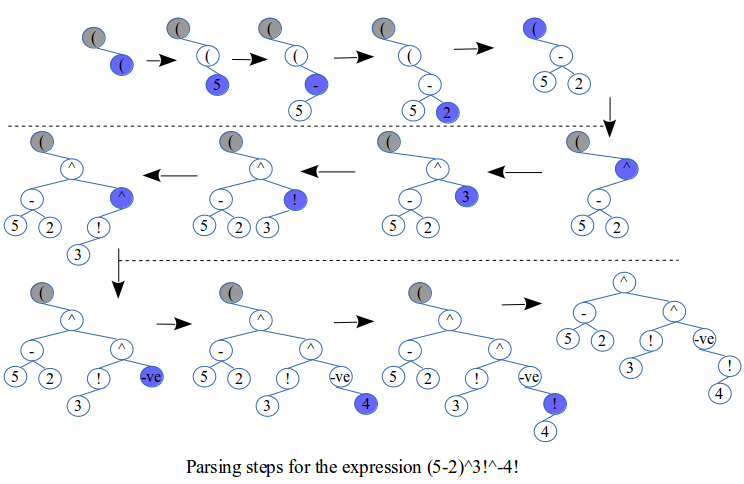
\includegraphics[width=\textwidth]{precAlgo.png}
        \end{column}
        \begin{column}{0.2\textwidth}
            \begin{array}{|c|c|}
                \hline
                (, ) & 1 \\
                \hline
                +, - & 2 \\
                \hline
                neg  & 3 \\
                \hline
                *, / & 4 \\
                \hline
                pow  & 5 \\
                \hline
                fact & 6 \\
                \hline
                const & max \\
                \hline
                fce & max \\
                \hline
            \end{array}
        \end{column}
    \end{columns}
\end{frame}

\begin{frame}{Algoritmus výpočtu podle Shunting yard algoritmu}
    \framesubtitle{zjednudušeně infix to RPN: eval = interpretace stacku RPN}
    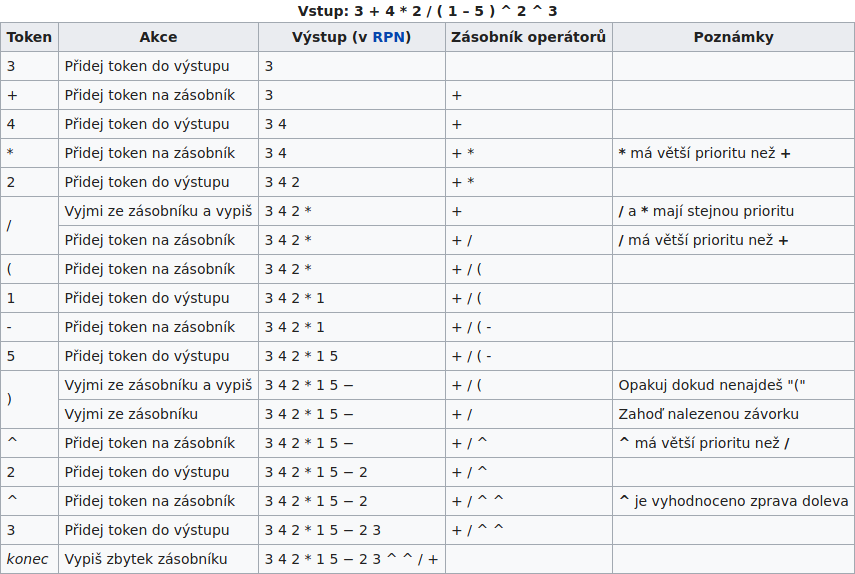
\includegraphics[height=0.8\textheight, keepaspectratio]{shunyardAlgo.png}
\end{frame}


\subsection{Obecně potřebné struktury pro řešení řetězcového zpracování}
\begin{frame}{Obecně potřebné struktury pro řešení řetězcového zpracování}
    \begin{itemize}
        \item Strom, při použití infix to ast algoritmu
        \item Stack, při použití Shunting yard algoritmu
    \end{itemize}
\end{frame}


\section{Přímý výpočet pomocí průběžných výpočtů}
\begin{frame}{Přímý výpočet (Immediate execution calculator)}
    \begin{block}{}
        2 registry: \\
        1. pro předešlý výsledek - ANS\\
        2. pro uchování zadaného čísla uživatelem
    \end{block}
    Operace budou zakotveny do tlačítek GUI a budou při klikání na operandy počítat průběžné výsledky. \\
    Veškerá logika programu se přesouvá do GUI frontendu. \\
    Při implementaci více funkcí/konstant univerza by mohlo dojít k znepřehlednění kódu a ke zhoršení přehlednosti frontendu aplikace.

\end{frame}

\begin{frame}{Reference:}
    infix to AST: \url{https://www.rhyscitlema.com/algorithms/expression-parsing-algorithm/}
\end{frame}

\end{document}

